\section{Photometric Properties}\label{sec:PhotProp}
\subsection{UV Luminosity Function}\label{sec:PhotProp.UVLF}
\begin{figure*}
	\centering
	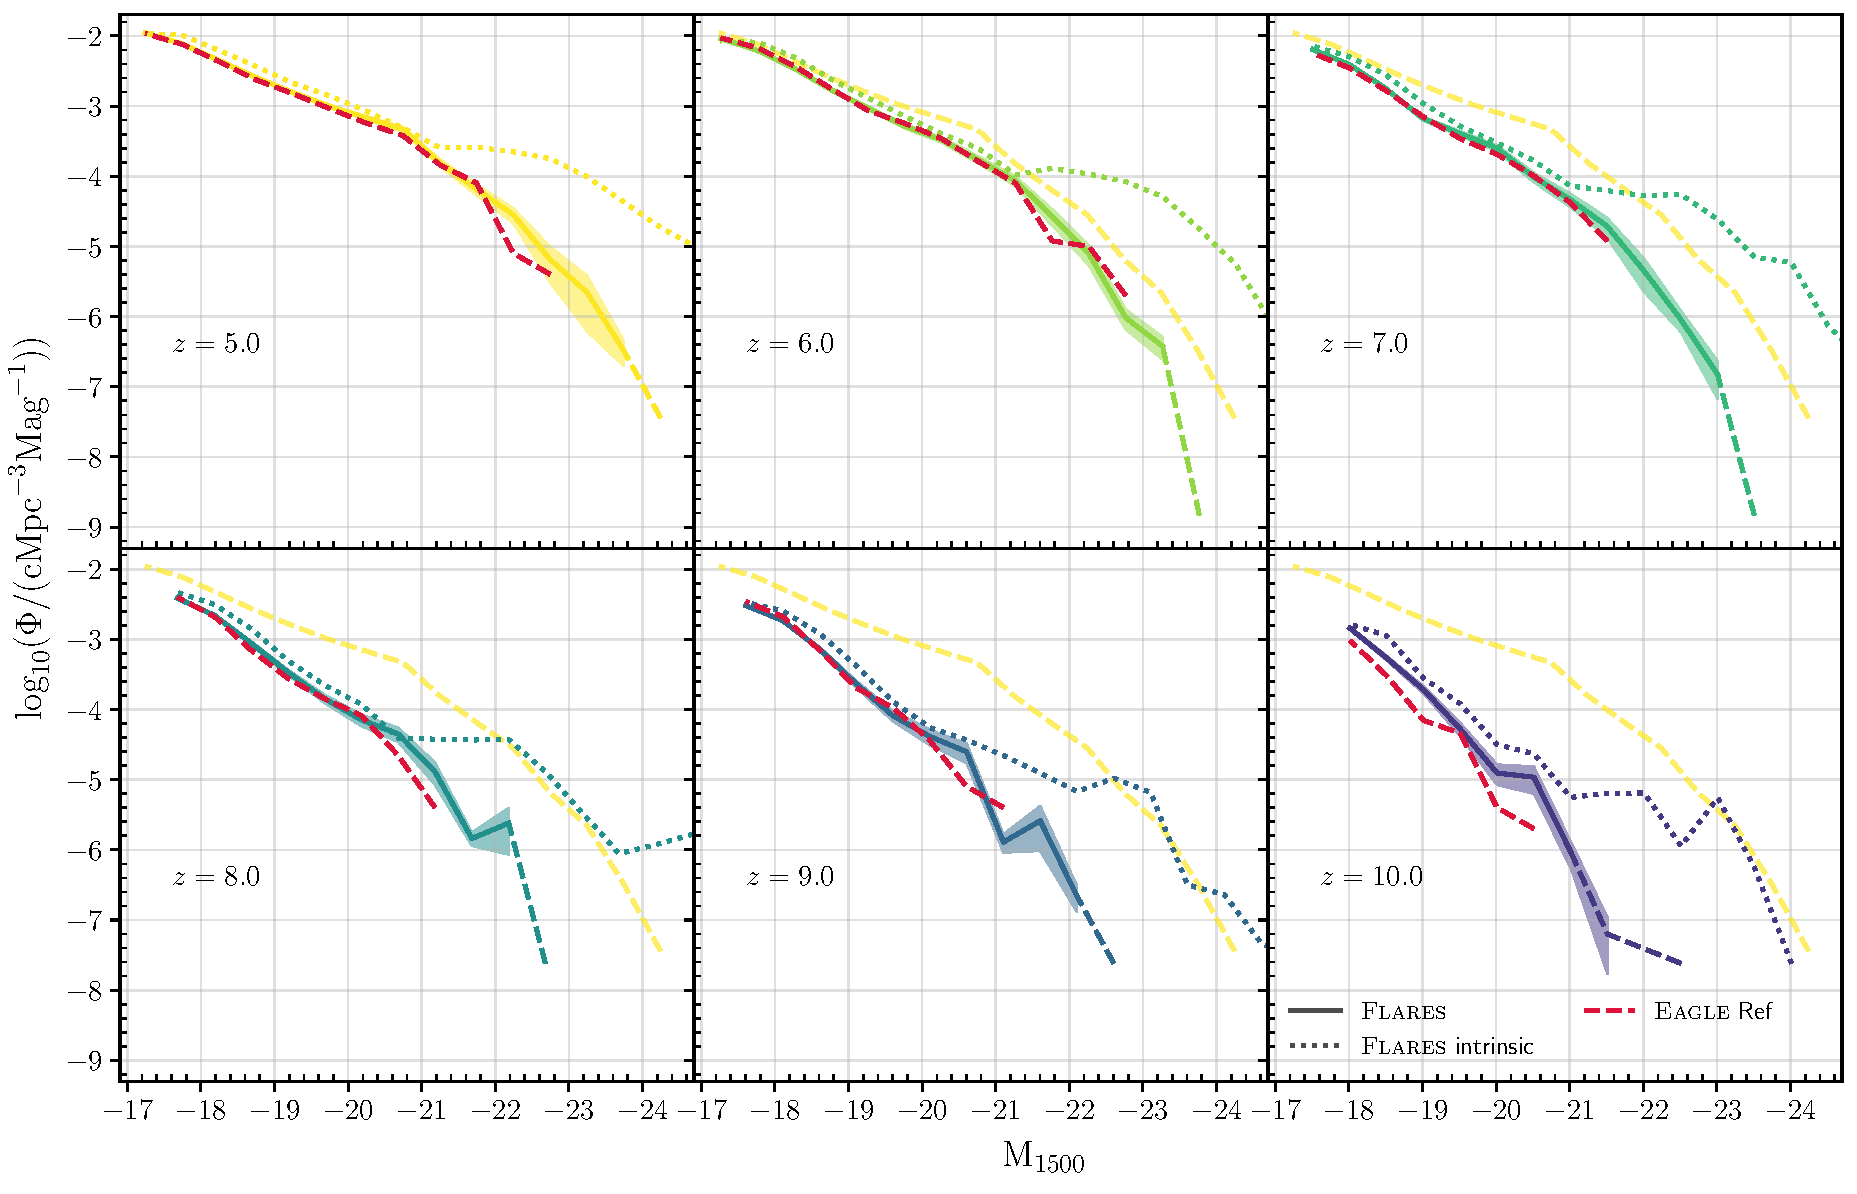
\includegraphics[width=\textwidth]{./figures/LF_FUV_z5_10_Flares-Eagle}
	\caption{\flares\, composite intrinsic (dotted) and dust attenuated (solid, dashed for bins with less than 3 \chris{people typically use at least 10, do we really have that few galaxies at the bright end?} galaxies) UV LF for  galaxies in z $\in$ [5,10]. Shaded region denote the poisson $1\sigma$ uncertainties for each bin from the simulated number counts for the \flares\, dust attenuated UV LF. For comparison the UV LF from the \textsc{Eagle} Reference volume is plotted. We also plot the $z=5$ dust attenuated UV LF (dashed line) alongside other redshifts for comparison. \label{fig: UVLF}} 
\end{figure*}
The UV LF evolution of high redshift galaxies is a regime where there are numerous observational studies done. We begin by calculating the rest-frame ultraviolet (UV) luminosity function (LF) of the \flares\, galaxies. 

\subsubsection{LF creation}\label{sec: UVLF.LF_creat}
Unlike the simulation of a periodic box the re-simulation strategy of \flares\, means that the creation of the luminosity function (or stellar mass function) is not straightforward. The contribution from any resim region needs to weighted by the appropriate weight for that region. The weighting strategy of \flares\, has been explained in detail in \S 2.3 in \citetalias{lovell2020}, we refer the readers there for more details. With the chosen values of $\kappa_{\textrm{BC}}=1.25$ and $\kappa_{\textrm{ISM}}=0.0063$ explained in \S\ref{sec:modelling.dust}, we present the obtained UV luminosity funtion of $z\in\,[5,10]$. 

This work as presented in \S\ref{sim.galident}, we concentrate on a more limited definition of a galaxy focusing on only those objects with a combined total of more than 100 gas and star particles, extending the stellar mass function to $\sim$ 10$^{7.5}$\Msun\, at $z=5$. For the luminosity function we set the low brightness cut-off for the selected galaxies to be the 97th percentile of the Magnitude computed for 100 gas and star particles \chris{I don't really get this, as your cut off will then surely evolve with the number of galaxies, which is constantly increasing, but isn't necessarily physical}, allowing us to probe down to $\sim$-17 in FUV rest-frame magnitude at $z=5$. 

\subsubsection{Luminosity Functions}\label{sec: PhotProp.UVLF.LF}
We plot the dust-attenuated (as described in \S\ref{sec:modelling.dust}) UV LF in Figure~\ref{fig: UVLF} (solid line) along with the intrinsic LF (dashed line). Here the plotted data for \flares\, are in bins of width 0.5Mags, with their 1 sigma Poisson scatter. Also plotted is the UV LF of the 100Mpc \eagle\, Reference simulation box.  It can be seen clearly that the luminosity function is extended to brighter galaxies by 2 Magnitudes or more at all redshifts, thus failing to probe the bright end of the UV LF. It is evident that at the faint-end the simulations agree. The bin centre and the number density per magnitude for the \flares\, galaxies are provided in Appendix~\ref{app: lum_func} as Table~\ref{tab: LF values}. 

The number density of bright galaxies increases by $\sim2$ orders of magnitude going from $5\to10$ in redshift, inidcating the rapid assembly of stars in galaxies through time. It can also be seen that the observed LF is slightly lower than the intrinsic LF at luminosities fainter than $\sim-20$. The reason for this is the implementation of a birth cloud component for young stellar populations. Studies of exploring the impact of birth cloud attenuation has shown that this can reduce the luminosities by $\sim\,0.3$ dex for galaxies in the local Universe \citep[\eg][]{Trayford2017}. Since the surface density of metals in the faint galaxies is insufficent to produce siginficant attenuation in the ISM, the choice of birth cloud component is most pronounced in this regime. While in the case of the bright end, the main contribution is from the dust attenuation in the ISM. 

It is important to take note that both these regimes can be affected by the choice of initial mass function, the SPS model \citep[see][]{Wilkins2016a} and the attenuation law. We also do not take into account the contribution of black hole accretion to the galaxy luminosity function; this could become important for the bright end, but is complicated to model (\comment{Steve could say something about this}).
\begin{figure}
	\centering
	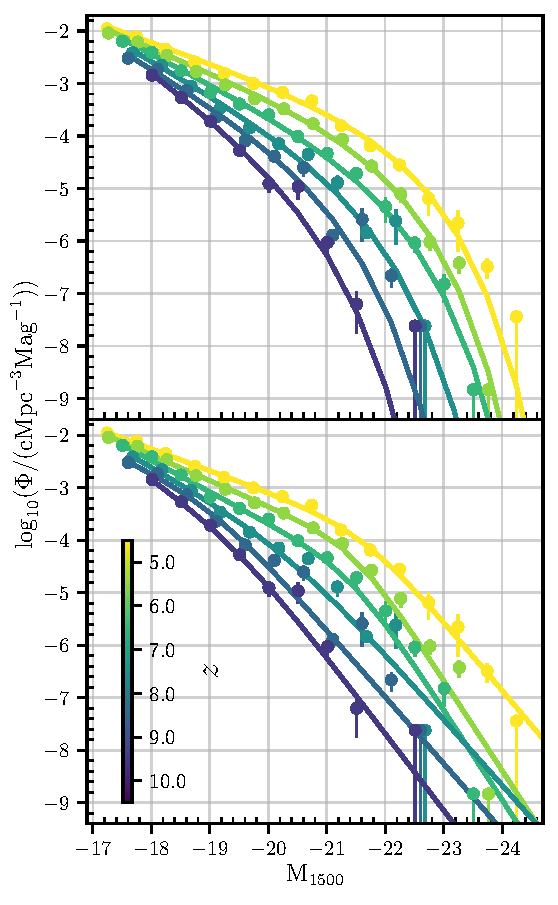
\includegraphics[width=\columnwidth]{./figures/LF_FUV_z5_10_Flares-fit}
	\caption{Schechter (top) and double power-law (bottom) fits to the \flares\, UV LF are plotted as solid lines while the data is shown as points with the error-bars denote the 1-$\sigma$ Poisson errors. \chris{Can't decide whether keeping the DPL fits in is worth it or not. They don't look great, even at $z = 7$ where they are supposedly 'better' according to BIC. Perhaps something is going wrong here} \label{fig: LF fit}} 
\end{figure} 
\begin{figure}
	\centering
	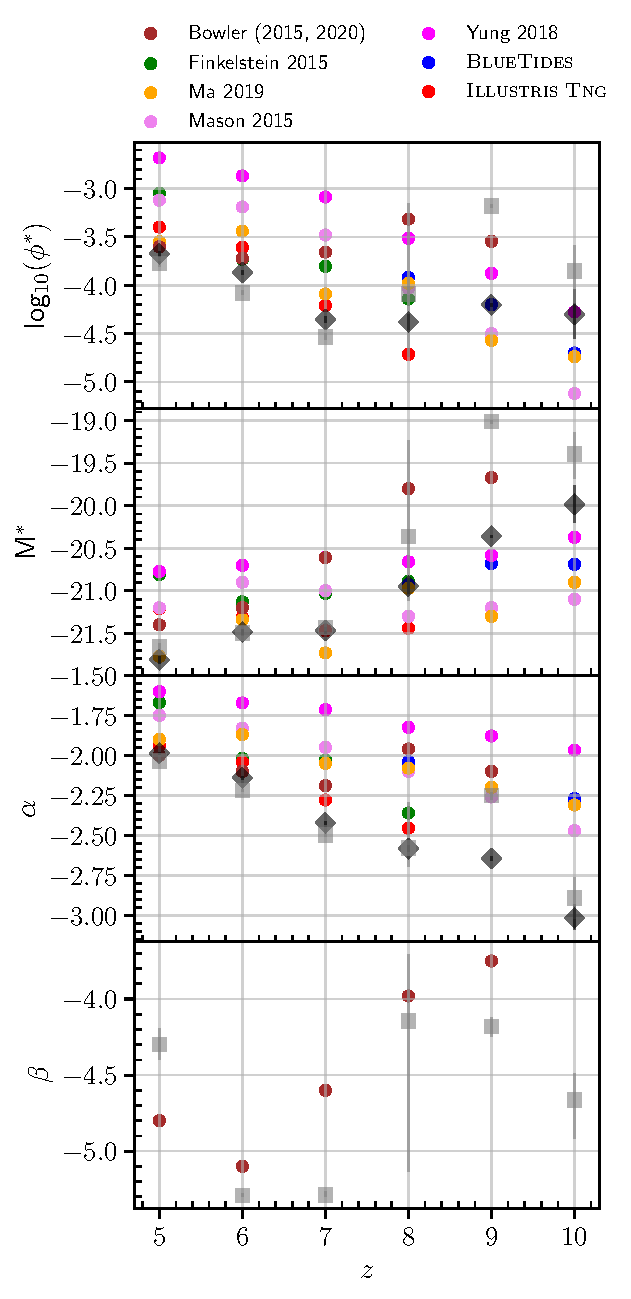
\includegraphics[width=\columnwidth]{./figures/fit_params_evo}
	\caption{Evolution of the parameters of Schechter (black diamonds) and double power-law (grey squares) fit to the \flares\, UV LF. Also plotted are the evolution of the Schechter fit parameters from \bluetides\,\protect\citep{Wilkins2017}, \protect\cite{Mason2015,Finkelstein2015,yung_semi-analytic_2019}; \textsc{Illustris Tng} \protect\citep[Model-C from][]{Vogelsberger2020} as well as the double power-law fit parameters from \protect\cite{Bowler2015,Bowler2020}. \label{fig: fit param evo}} 
\end{figure}

The observed UVLF can be described by a Schechter function \citep[\eg][]{Bouwens_2015a,Finkelstein2015}, characterized by a power law at the faint end with slope $\alpha$, with an exponential cutoff at the bright end at a characteristic magnitude M$^*$, with the parameter $\phi^*$ setting the normalization of this function. The number density at a given magnitude is then given by
\begin{equation}\label{eq: schechter}
\phi(M) = 0.4\,\text{ln}\,10\,\phi^{*}\,10^{-0.4(M-M^*)(\alpha+1)}\,e^{-10^{-0.4(M-M^*)}} 
\end{equation}
To provide an easier comparison with other work we also calculate the Schechter function parameters of our LFs (see Appendix \ref{app: lum_func} for more details of the fitting). The Schechter fits to the UV LF of \flares\, galaxies is shown in Figure~\ref{fig: LF fit} (left panel). We find that the function provides a good fit to the shape of the overall UV LF. The best-fitting schechter parameters to the UVLF are shown in Table~\ref{tab: fit params}. It should be noted that in case of $z=9,10$ we set narrow priors for M$^*$, which was done by visual inspection.

There has also been some studies that has shown a double power-law can also be used to describe the shape of the UV LF at higher redshifts \citep[\eg][]{Bowler2014}. The parameterization for a double power-law is as follows
\begin{equation}\label{eq: DPL}
	\phi(M)  = \frac{\phi^*}{10^{0.4(M-M^*)(\alpha+1)} + 10^{0.4(M-M^*)(\beta+1)}}
\end{equation}
where $\alpha$ and $\beta$ are the faint-end and bright-end slopes,
respectively, M$^*$ is the characteristic magnitude between these two power-law regimes, and $\phi^*$ is the normalisation. The double power-law fit to the binned luminosities is shown in Figure~\ref{fig: LF fit} (right panel). The best-fitting double power-law parameters to the UVLF are also shown in Table~\ref{tab: fit params}. It can be seen that this also provides a good fit to the UV LF eventhough it can overestimate the number density at the brightest end for $z<7$.

We have already shown in \citetalias{lovell2020} that the galaxy stellar mass function follows a double Schechter shape in \flares. It can be seen in Figure~\ref{fig: UVLF} that the intrinsic UV LF also has a double Schechter shape, but the observed UV LF does not. It lies much closer to a Schechter or a double power-law shape depending on the redshift in \flares. This can be explained by dust attenuation suppressing the intrinsically bright galaxies at the knee and beyond. Also shown is the evolution of the parameters of the Schechter and double power-law fits with redshift in Figure~\ref{fig: fit param evo}. We see that for both the fit functions, the value of M$^*$ and $\alpha$ are similar across redshift, with the values generally decreasing with redshift for M$^*$ and vice versa for $\alpha$. 

We compare the performance of the two functional forms across redshifts by computing the Bayesian Information Criterion \citep[BIC, see][and references therein for further details; also see Appendix~\ref{app: lum_func}]{Schwarz1978,Liddle2007} for the best-fit parameters. 
A model with a lower BIC is preferred. For this purpose we give the difference between the BIC values of the double power-law and the Schechter best-fit values, which is also quoted in Table~\ref{tab: fit params}. As can be seen a double power-law function is a much better fit to the UV LF of the \flares\, galaxies at redshifts $z=5,9,10$. Some studies of the observational data \citep[\eg][]{Bowler2014,Bowler2020} have suggested that there is not much evolution in the bright end of the galaxy luminosity function because of the lack of quenched galaxies at these redshifts, favouring a double power-law fit to the population. The bright end is very dependent on the dust content as well as star formation of the galaxies, and thus also provides constraints on the recipes of dust modelling and star formation. None of the \flares\, regions have galaxies that moved into the passive regime at $z>6$, thus it is not surprising that the double power-law is preferred at the higher redshifts. 


\subsubsection{Comparison with Observations and Models}\label{sec: PhotProp.UVLF.Compare}
\begin{figure*}
	\centering
	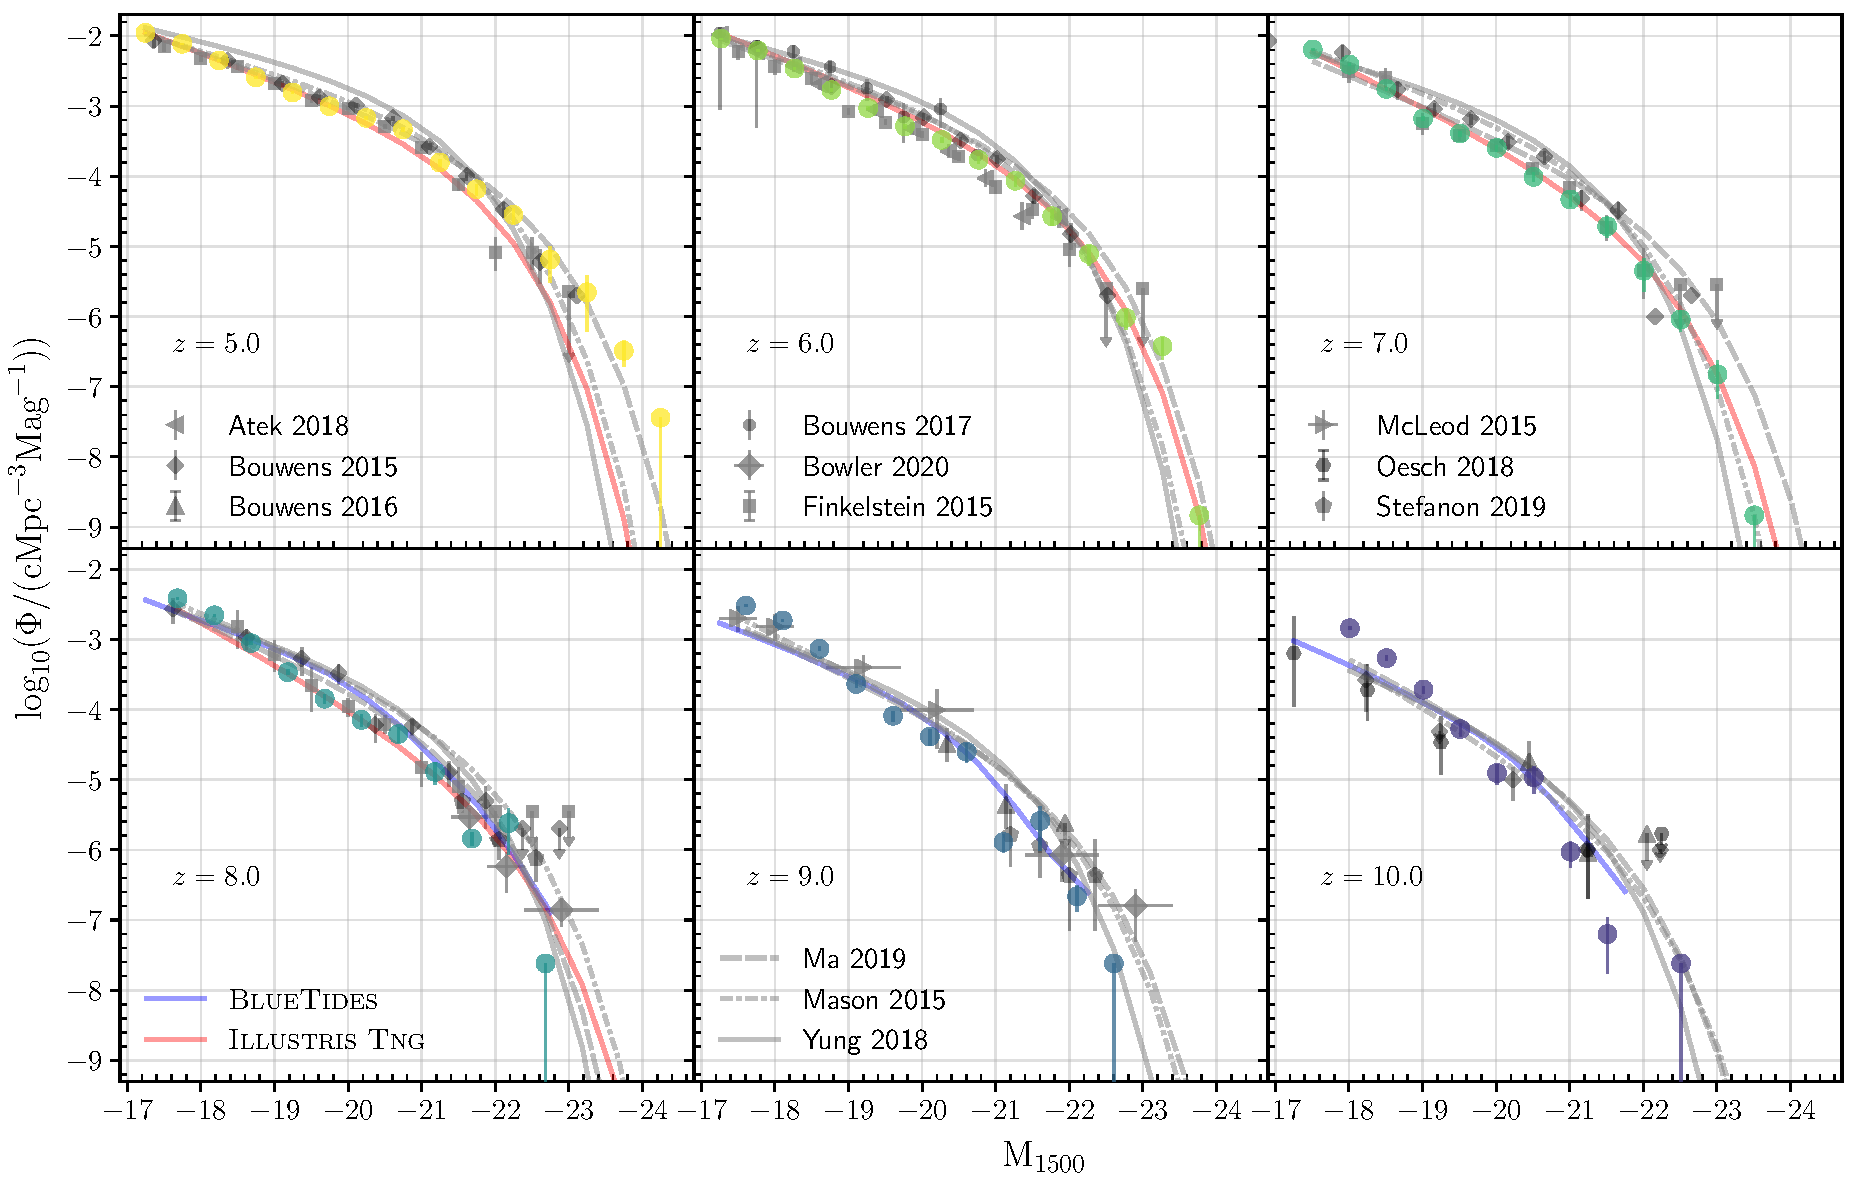
\includegraphics[width=\textwidth]{./figures/LF_FUV_z5_10_Observations+Models}
	\caption{UV LF for \flares\, galaxies, with the corresponding Schechter (coloured solid) and double power-law (coloured dashed) fit is plotted for z $\in$ [5,10]. Error bars denote the poisson $1\sigma$ uncertainties for each bin from the simulated number counts for the \flares\, dust attenuated UV LF. Observational data from \protect\cite{Bouwens_2015a,McLeod2015,Finkelstein2015,Bouwens_2016,Bouwens2017,Oesch_2018,Atek2018,Stefanon2019,Bowler2020} are plotted as well as the binned luminosities from \bluetides\,\protect\citep{Wilkins2017} and the Schechter fits from \protect\cite{Mason2015,ma_dust_2019, yung_semi-analytic_2019}; \textsc{Illustris Tng} \protect\citep[Model-C from][]{Vogelsberger2020} are shown for comparison.  \label{fig: UVLF Compare}} 
\end{figure*}
In Figure~\ref{fig: UVLF Compare} the UV LF of \flares\, galaxies is compared to observational values from
\cite{Bouwens_2015a,McLeod2015,Finkelstein2015,Bouwens_2016,Bouwens2017,Oesch_2018,Atek2018,Stefanon2019,Bowler2020}. The Schechter as well as the double power-law fit to the \flares\, population is also shown. 

We predict the UV LF relation at all redshift well in comparison to the observations, while slightly underpredicting the luminosities of galaxies as we progress to higher redshifts. But it should also be noted that the uncertainties in the observations gets progressively larger with increasing redshift and some of the number densities at the bright end are upper limits.

In Figure~\ref{fig: UVLF Compare}, we also plot the binned luminosities from \bluetides\,\citep{Wilkins2017} and the Schechter function fits from \cite{Mason2015}, \textsc{Fire-2} \citep{ma_dust_2019}; \textsc{SantaCruz} SAM \citep{yung_semi-analytic_2019}; \textsc{Illustris Tng} \protect\citep[Model-C from][]{Vogelsberger2020}. As can be seen the fit is similar to others from literature, and only starts to diverge slightly at $z\ge8$, with \flares\, having a lower number density at the bright end compared to the Schechter fits from \cite{Mason2015,ma_dust_2019}. Modelling differences across the studies or the larger dynamic range probed by \flares\, is a possible explanation for this deviation. With respect to \bluetides\,, a comparison of data have shown us that the most massive galaxies in \flares\, are more metal rich by $\sim$0.1dex. 

In Figure~\ref{fig: fit param evo} we also plot fit paramters from other studies of simulations \citep{Mason2015,Wilkins2017,yung_semi-analytic_2019,Vogelsberger2020} as well as observations \citep{Finkelstein2015,Bowler2015,Bowler2020}.  There exists degeneracies between the fit parameters \citep[\eg][]{Robertson2010a}, and depends upon the dynamic range and the statistics of the galaxy population. Thus it is not straightforward to compare different studies. From Figure~\ref{fig: fit param evo}, it can be seen that the \flares\, functional parameters roughly matches the trend exhibited by the various simulation as well as observational data. The difference in the fit parameters 

%\begin{figure}
%	\centering
%	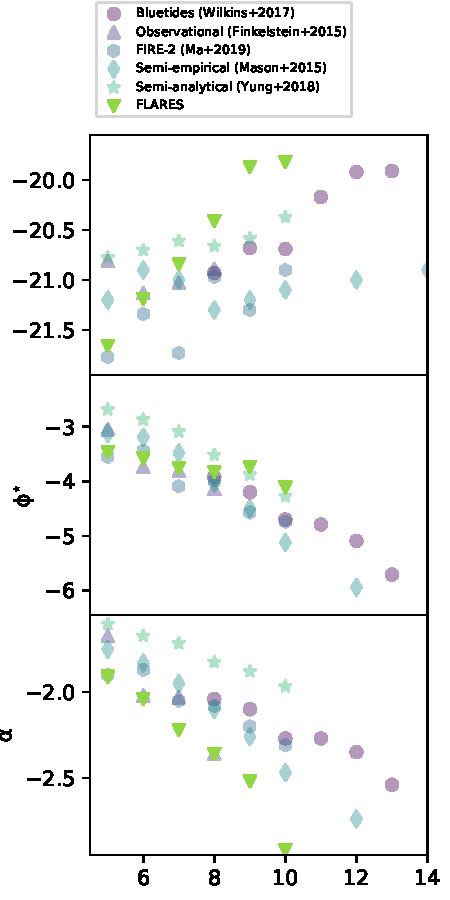
\includegraphics[width=0.4\textwidth]{./figures/LF_parameters_models}
%	\caption{Comparison of our schechter fit parameters for UV luminosity function against values from other studies.\label{fig: UVLF params}} 
%\end{figure}

\subsubsection{Effect of environment on UV LF}\label{sec: PhotProp.UVLF.Env}

\begin{figure*}
	\centering
	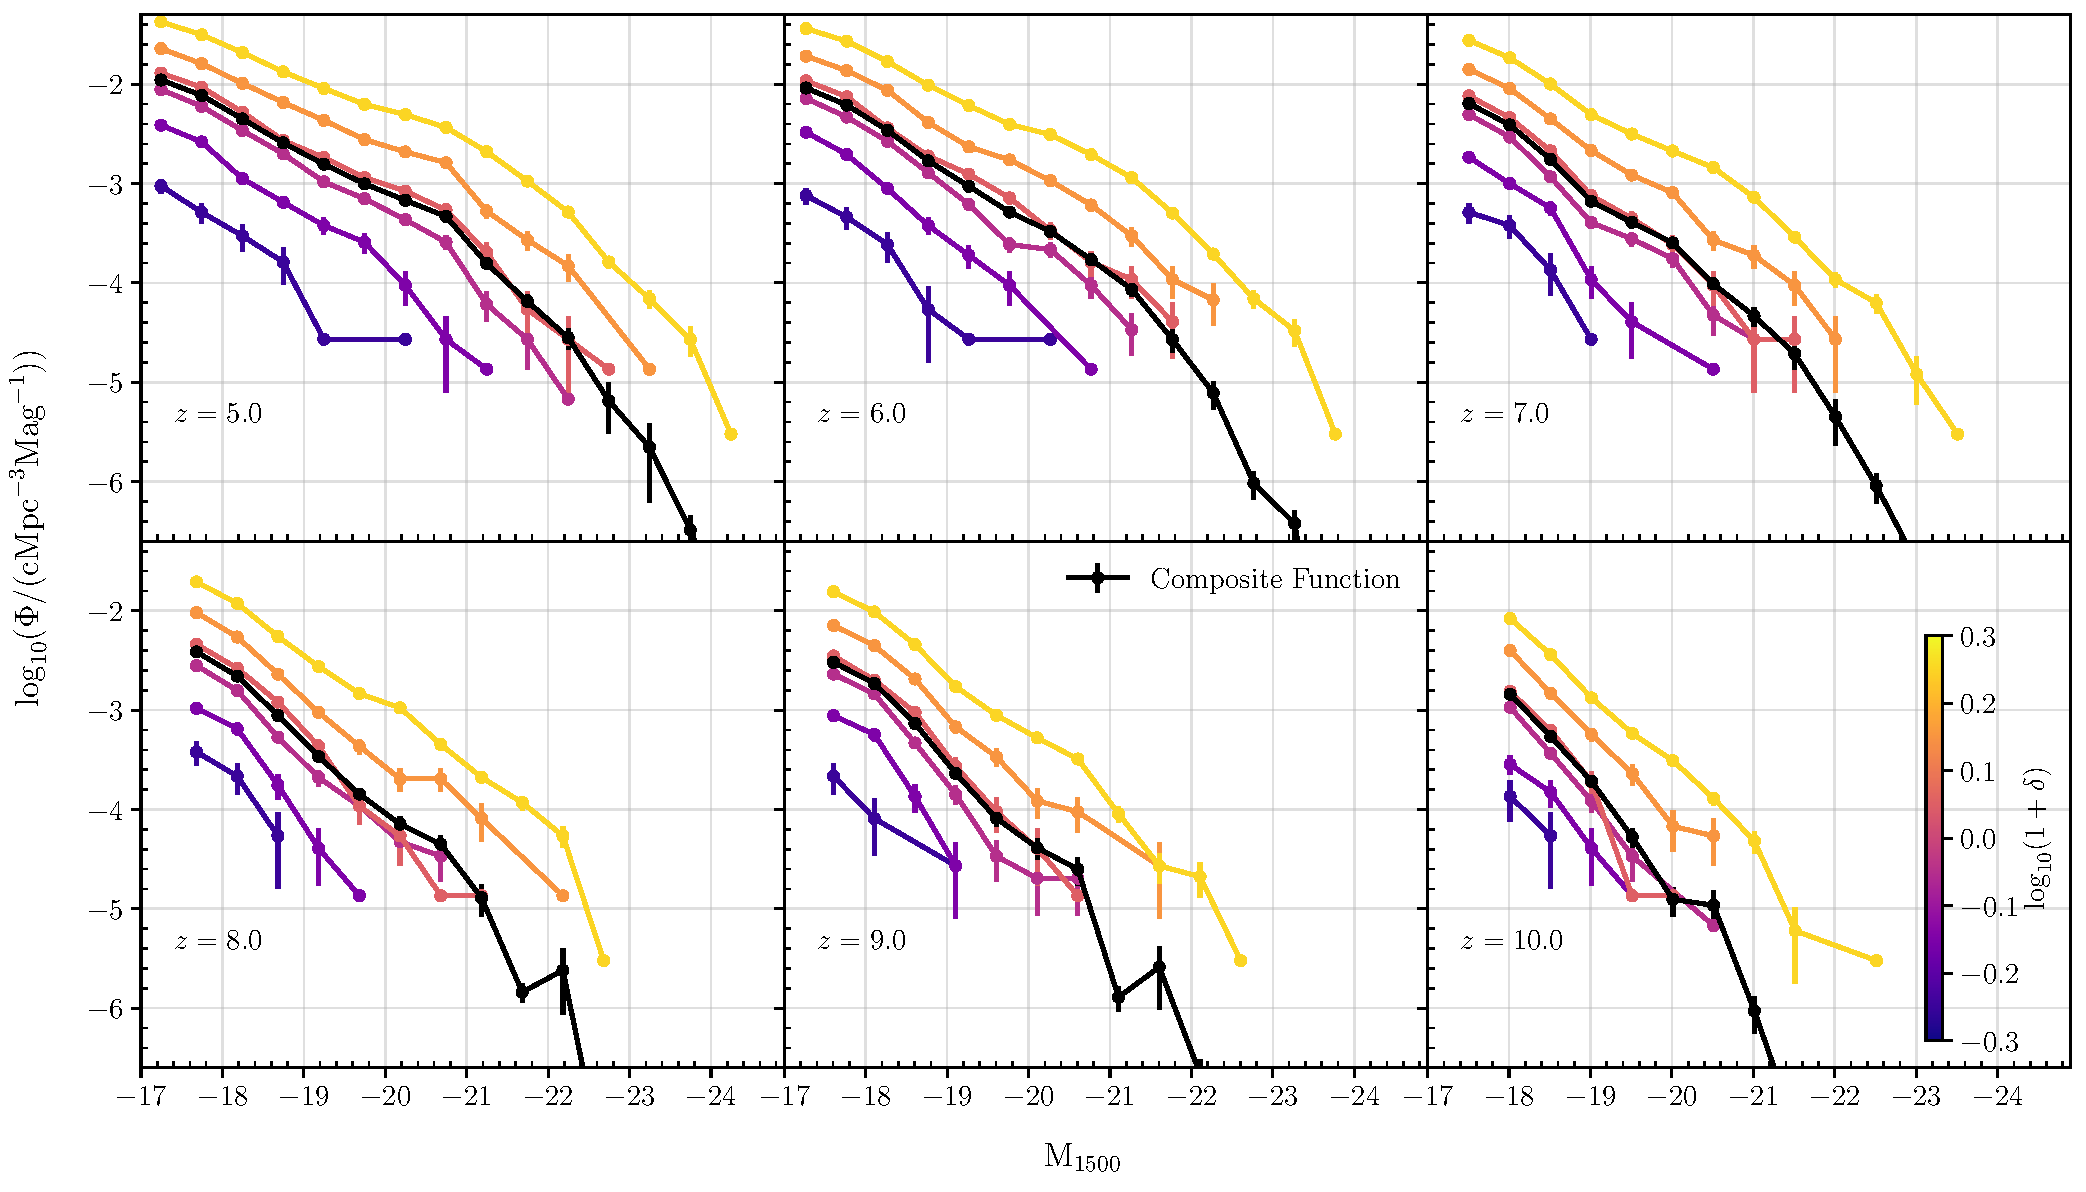
\includegraphics[width=\textwidth]{./figures/UVLF_env}
	\caption{The \flares\, UVLF for $z \in [5,10]$ split by
		binned log-overdensity. Error bars denote the poisson $1\sigma$ uncertainties for
		each bin from the simulated number counts. \label{fig: UVLF env}} 
\end{figure*}
The \flares\, simulation probes galaxies that reside in a wide range of environments allowing us to analyse the effect environment has on their properties. In Figure~\ref{fig: UVLF env} we look at how the UV LF varies as a function of overdensity for $z \in [5,10]$. Here we have plotted the UV LF in 6 bins of log$_{10}$($1+\delta$), where $\delta$ is the overdensity. As expected the number of galaxies increases with increasing overdensity and the brighter galaxies reside in denser environments. The normalization shows a variation of $\sim2$ dex from the low to the highest density environment probed in \flares. The composite distribution function follows closely the mean density region as expected, in the regimes below the bright end, with the contribution to the bright end only coming from the densest environments. 

As can be seen from Figure~\ref{fig: UVLF env} the shape of the luminosity function is similar across various environments with the knee of the function shifting to fainter magnitudes with decreasing density. In the intermediate environments there is a hint of a double power-law shape while the densest regions follow a Schechter shape. This could be due to the dearth of galaxies being sampled in the lower density environments or due to different assembly histories of galaxies driven by the environment. The effect of environment on assembly history as well as on astronomical surveys will be probed in a future work (Thomas et al. in prep). 

%The difference seen in the Schechter fit parameters presented in Figure~\ref{fig: UVLF params}, compared to observational studies as well as other models could be attributed to us probing higher densities thus having a better sampling of the bright end as well the knee of the function.

\subsection{UV continuum slope ($\beta$)}\label{sec: PhotProp.beta}
\begin{figure*}
	\centering
	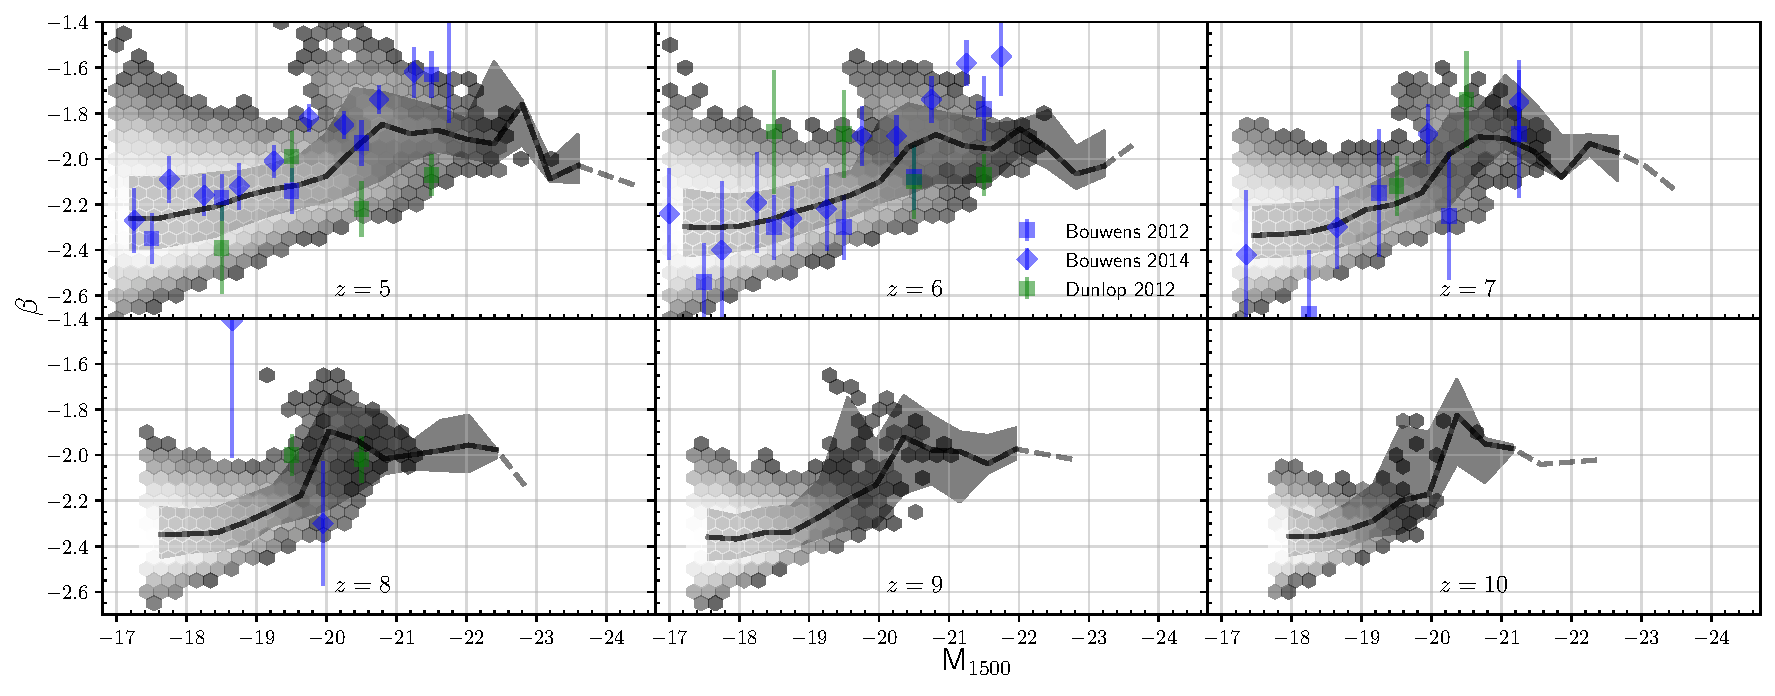
\includegraphics[width=\textwidth]{./figures/beta_lum_z5_10}
	\caption{UV-continuum slope, $\beta$ is plotted against the UV magnitude for $z\in[5,8]$. The solid dashed line is the weighted median of the sample, with the shaded region indicating the weighted 84 and 16 percentiles. The hexbin denotes the distribution of our sample, only plotted are bins with more than 5 data points. Plotted alongside are bservational values from \protect\cite{Dunlop2012,Bouwens2012b,Bouwens2014a}.\label{fig: beta}} 
\end{figure*} 
\begin{figure*}
	\centering
	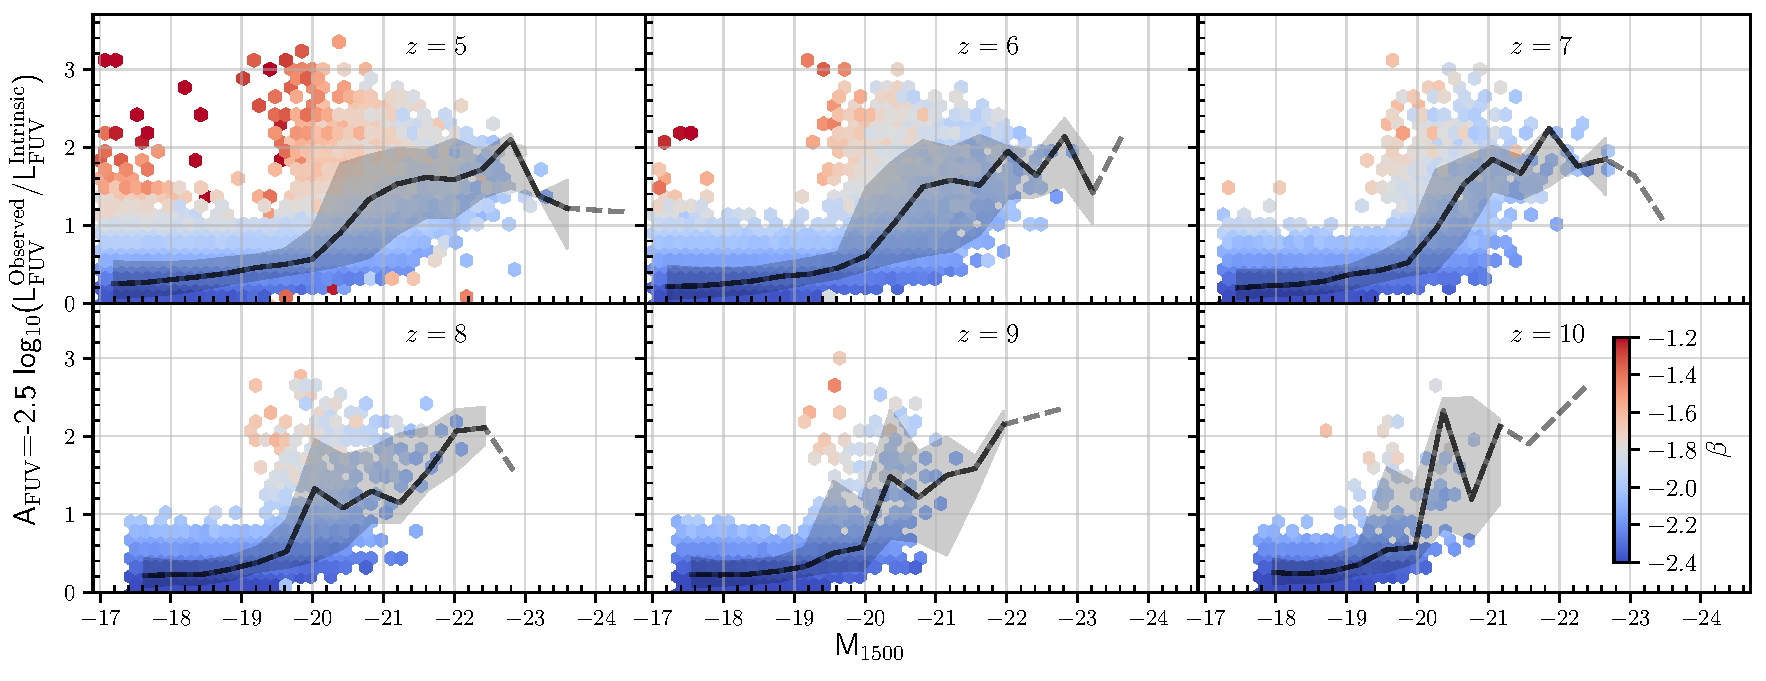
\includegraphics[width=\textwidth]{./figures/att_lfuv_beta_z5_10}
	\caption{The attenuation in the FUV is plotted against the observed UV magnitude for $z\in[5,10]$. The solid and dashed black line is the weighted median of the sample, with the shaded region indicating the weighted 84 and 16 percentiles. The dashed line is for bins that have less than 3 data points. The hexbin denotes the distribution of our sample, coloured by the median $\beta$ value in the hexbin. \label{fig: att_lfuv}} 
\end{figure*} 
\begin{figure*}
	\centering
	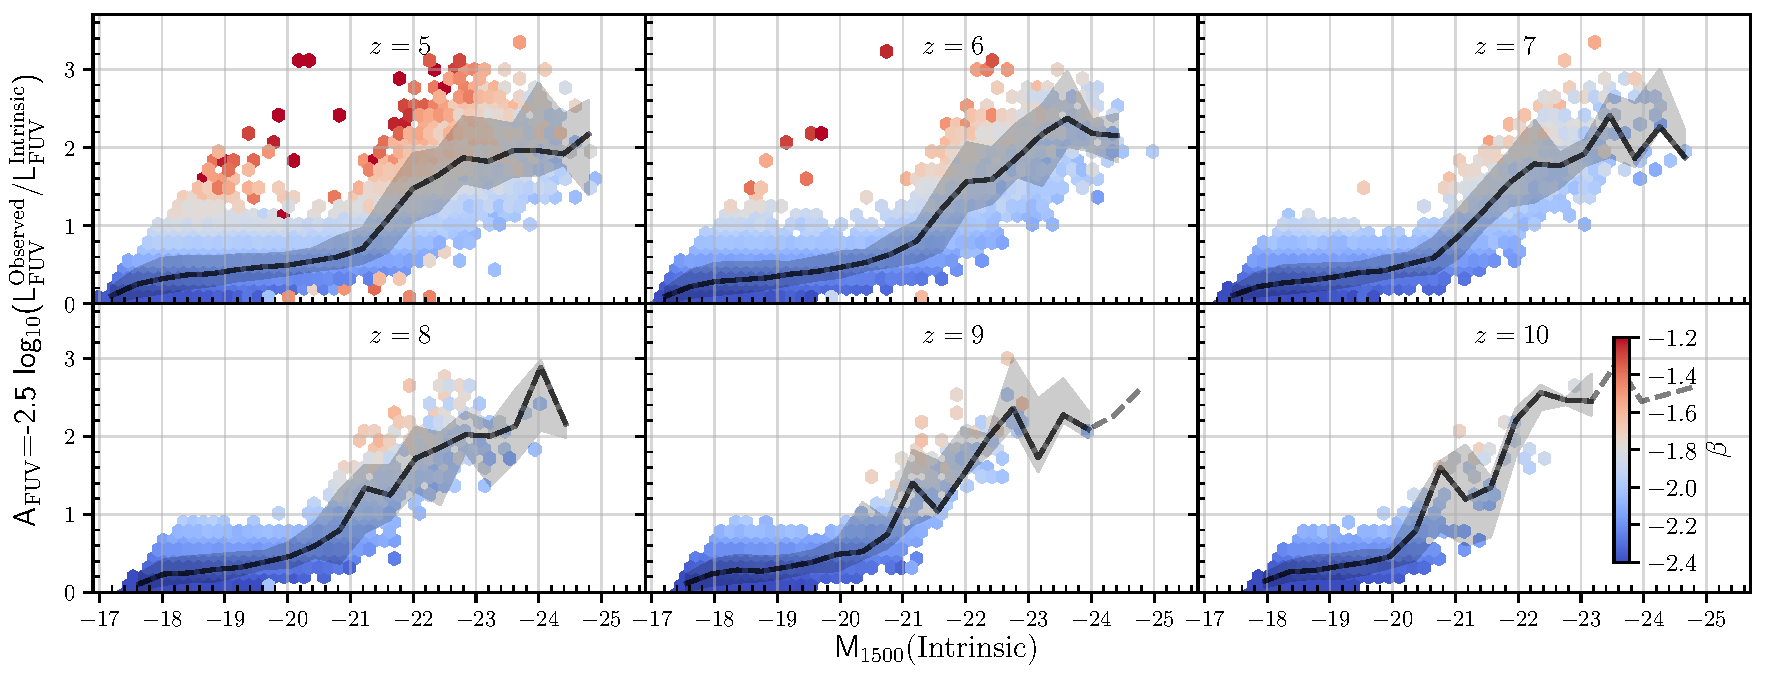
\includegraphics[width=\textwidth]{./figures/att_lfuvintr_beta_z5_10}
	\caption{The attenuation in the FUV is plotted against the intrinsic UV magnitude for $z\in[5,10]$. The solid and dashed black line is the weighted median of the sample, with the shaded region indicating the weighted 84 and 16 percentiles. The dashed line is for bins that have less than 3 data points. The hexbin denotes the distribution of our sample, coloured by the median $\beta$ value in the hexbin. \label{fig: att_lfuv_intrinsic}} 
\end{figure*} 
The UV continuum slope $\beta$, defined such that f$_{\lambda}\,\propto\,\lambda^{\beta}$, commonly used as a tracer of the stellar continuum attenaution. At high reshifts the rest-frame UV becomes accessible to optical/near-IR instruments. This has been studied by different groups (citations) as it is available due to deep near-IR observations using the Wide Field Camera 3 (WFC3) on the \textit{Hubble Space Telescope}. These studies have shown that $\beta$ is particularly sensitivity to the metallicity, age, and especially the dust content within a galaxy, and thus it is a useful quantity to check the reliability of theoretical models. But it is important to note that $\beta$ is also strongly dependent the modelling assumption in theoretical studies like the choice of the IMF, SPS model, dust modelling and extinction law.   

Figure~\ref{fig: beta} plots the value of $\beta$ against the UV luminosity of the galaxies in \flares. Observational values of $\beta$ from \cite{Dunlop2012,Bouwens2012b,Bouwens2014a} are plotted alongside for comparison. It should be noted that the observational data shows a lot of scatter and the different datasets does not show the same trends. Our weighted median of $\beta$'s  match observational values for almost all luminosities. At the bright end, M$_{1500}<-20$ the \cite{Bouwens2012b,Bouwens2014a} data predict much steeper $\beta$'s compared to our results, which start to flatten while \cite{Dunlop2012} shows lower values. This could be due to the choice of our extinction curve, a steeper/shallower curve will make for a steeper/shallower relation. The $\beta$ values are an excellent constrain on the theoretical extinction curves, giving insights into the dust properties within the galaxy \citep[see][for an overview]{Salim2020}. We try a few extinction curves from literature (namely the Calzetti \citep{Calzetti2000}, Small Magellanic Cloud \citep{Pei1992} and the curve used in \citealt{Narayanan2018}) in Appendix~\ref{app:extinction_curves} and plot the effect it has on the  UV-continuum relation in Figure~\ref{fig: ext curves beta}. 

In Figure~\ref{fig: att_lfuv} we plot the attenuation in the FUV against the FUV luminosity, in hexbins coloured by the median $\beta$ value. Overall, brighter galaxies suffer more attenuation, which is expected as they have had more time to produce stars thus enriching the ISM. The figure also shows that many of the galaxies at the bright end are not the most attenuated ones. These are the galaxies that have enjoyed a recent burst of star formation and have not had the time to enrich the ISM with dust. Another possible explanation is that there might be star particles in our simulation that reside in lines-of-sight that suffer little to no dust extinction making them bright. Another alternative is stellar migration \citep[see][]{furlong_evolution_2015}, with some stars moving radially outwards, and thus could suffer less effects of dust depending on the viewing angle or geometry. This is evident from Figure~\ref{fig: att_lfuv_intrinsic} where we plot the attenuation as a funcion of intrinsic FUV luminosity. Now this plots provide more insights into the features seen in Figure~\ref{fig: att_lfuv}; that in general intrinsically brighter galaxies are more attenuated. A comparison also reveals that the intrinsically bright galaxies, since they are too dusty, many of them are not the brightest galaxies observed in the UV. We also plot attenuation as a function of galaxy stellar mass in Figure~\ref{fig: att_Mstar} and a similar feature can be seen there as well. 

We have looked at the few galaxies at $z=5$ that have very low attenuation but are intrinsically bright and having a high $\beta$ value. These are galaxies that are identified to be in the passive regime whose specific star formation rate was calculated to be $\lesssim$ 1/(3$\times$H(z)), where H(z) is the Hubble constant at $z=5$. We will be studying this population in more detail in a future work (Wilkins et al. in prep). 

